% Graphics for slide 5, in the order the PDF draws them.
\begin{tikzpicture}[remember picture, overlay, x=1bp, y=-1bp,
  shift={(current page.north west)}]
\path[fill=cFFFFFF] (0,0) rectangle (960,540);
\path[fill=cF2F2F2,even odd rule] (674.25,69.28) ..controls(674.25,62.43)and(679.8,56.88)..(686.66,56.88) --(890.22,56.88) ..controls(897.07,56.88)and(902.62,62.43)..(902.62,69.28) --(902.62,444.72) ..controls(902.62,451.57)and(897.07,457.13)..(890.22,457.13) --(686.66,457.13) ..controls(679.8,457.13)and(674.25,451.57)..(674.25,444.72) --(674.25,69.28);
\node[anchor=north west, inner sep=0pt] at (674.25,56.88) {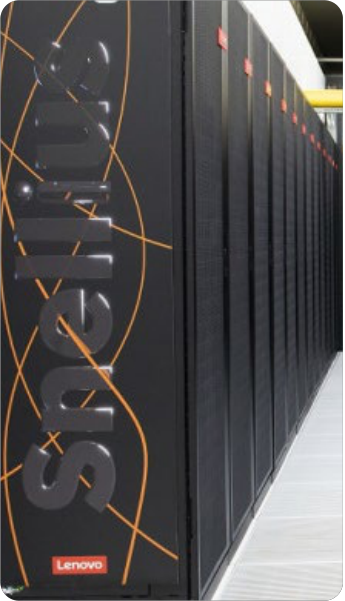
\includegraphics[width=229.31bp, height=400.28bp]{figures/fundamentals-of-hpc/p05-1.png}};
\node[anchor=north west, inner sep=0pt] at (56.69,477.21) {
\includegraphics[width=73.42bp, height=37.42bp]{figures/fundamentals-of-hpc/p03-1.png}};
\path[fill=cEE7628,even odd rule] (57.18,55.73) ..controls(57.96,55.73)and(58.6,56.37)..(58.6,57.15) --(58.6,85.5) ..controls(58.6,86.28)and(57.96,86.91)..(57.18,86.91) ..controls(56.4,86.91)and(55.76,86.28)..(55.76,85.5) --(55.76,57.15) ..controls(55.76,56.37)and(56.4,55.73)..(57.18,55.73);
\node[anchor=north west, inner sep=0pt] at (672.96,431.04) {
\includegraphics[width=137.64bp, height=32.76bp]{figures/fundamentals-of-hpc/p05-3.png}};
\end{tikzpicture}
